\documentclass[parskip=full]{scrartcl}
\usepackage[utf8]{inputenc} % use utf8 file encoding for TeX sources 

\usepackage[T1]{fontenc} % avoid garbled Unicode text in pdf 
\usepackage[german]{babel} % german hyphenation, quotes, etc 
\usepackage{hyperref} % detailed hyperlink/pdf configuration
\usepackage{graphicx}
\usepackage[toc]{glossaries}
\usepackage{caption}
\hypersetup{ % ‘texdoc hyperref‘ for options 
pdftitle={PSE Pflichtenheft}, %
bookmarks=true,%
}
\usepackage{csquotes} % provides \enquote{} macro for "quotes"
\usepackage{enumitem}




\makeglossaries
\newglossaryentry{Schachregeln}
{
	name=Schachregeln,
	description={Schachregeln die gültige Züge und das Ende des Spiels definieren. https://de.wikipedia.org/wiki/Schach\#Spielregeln}
}

\newglossaryentry{Schach}
{
	name=Schach,
	description={Das Brettspiel Schach}
}

\newglossaryentry{Schachfigur}
{
	name=Schachfigur,
	description={Die Spielsteine auf einem Schachbrett},
	plural=Schachfiguren
}

\newglossaryentry{Schachbrett}
{		
	name=Schachbrett,
	description={Das Spielbrett. Es ist quadratisch, zweifarbig und besteht aus 64 quadratischen Kacheln. Diese besitzen alle dieselbe Größe und sind in waagrechter und senkrechter Richtung abwechselnd eingefärbt},
	plural=Schachbretter
}

\newglossaryentry{Ausgangsposition} 
{
	name=Ausgangsposition,
	description={Vorgeschriebene Startposition aller Spielfiguren zu Beginn jeder Schachpartie}
}

\newglossaryentry{Remis}
{
	name=Remis,
	description={Der unentschiedene Ausgang einer Schachpartie, entweder durch Einigung beider Spieler oder durch Erreichen einer Stellung oder Zugfolge, welche ein Unentschieden erzwingt}
}

\newglossaryentry{Spieler}
{
	name={Spieler},
	description={Ein Nutzer der App},
}

\newglossaryentry{Elo}
{
	name={Elo},
	description={Wertung, die die Spielstärke beschreibt. https://de.wikipedia.org/wiki/Elo-Zahl}
}

\newglossaryentry{Schachmatt}
{
	name={Schachmatt},
	description={Der König steht im Schach und es gibt keinen regelkonformen Zug der das Schachgebot aufhebt. https://de.wikipedia.org/wiki/Schachmatt}
}
\newglossaryentry{Android}
{
	name={Android},
	description={Ein Betriebssystem für mobile Geräte wie Smartphones, Tablets und auch Fernseher}
}
\newglossaryentry{Smartphone}
{
	name={Smartphone},
	description={Ein Mobiltelefon mit umfangreichen Computer-Funktionalitäten},
	plural = Smartphones
}
\newacronym{GUI}{GUI}{Graphical User Interface}



\begin{document}
	\begin{titlepage}
		\centering
		\vspace*{0.2\textheight}
		{\Large PSE}\\[\baselineskip]
		{\Huge PFLICHTENHEFT}\\[\baselineskip]\par
		{\LARGE Rukiye Devran, Tim Groß, Daniel Helmig, Orkhan Aliev, Florian Weber}\par
	
	\newpage	
	\tableofcontents
	\pagebreak
	
	\end{titlepage}
\section{Einleitung}
\section{Zielbestimmung}
Es soll eine App angeboten werden mit der Personen gegeneinander \gls{Schach} spielen können. \gls{Spieler} sollen durch eine Spielersuche andere Gegner finden und können sich in einer Rangliste vergleichen. 
\subsection{Musskriterien}
\begin{description}
\item[KM1010] Alle \gls{Schachregeln} müssen implementiert werden.
\item[KM1020] Der \gls{Spieler} muss gemäß den \gls{Schachregeln} spielen.
\item[KM1030] Es muss eine Spielersuche geben.
\item[KM1040] Es muss eine \gls{GUI} existieren.
\item[KM1050] Es müssen die \glspl{Schachfigur} angetippt und bewegt werden.
\end{description}

\subsection{Wunschkritierien}
\begin{description}
\item[KW1010] Es soll einen Account/Gastzugang geben.
\item[KW1020] Der \gls{Spieler} kann ein Spiel nach dem beenden speichern.
\item[KW1030] Der \gls{Spieler} kann eine Bedenkzeit einstellen.
\item[KW1040] \gls{Spieler} können einen Chat mit dem entsprechenden Gegner führen.
\item[KW1050] Es soll ein Leaderboard oder ein \gls{Elo}system geben.
\item[KW1060] Die Anmeldung kann mit Facebook oder Google getätigt werden.
\item[KW1070] Es können zwei \gls{Spieler} auf einem Gerät gleichzeitig spielen.
\item[KW1080] Es soll einen Revanche-Button geben.
\item[KW1090] Es soll verschiedene Spielvarianten geben.
\end{description}
\subsection{Abgrenzkriterien}
\begin{description}
\item[KA1010] Es soll keine selbstspielende Schach-Engine implementiert werden.
\item[KA1020] Die Spieler können Züge nicht zurücknehmen.
\item[KA1030] Bei der Spielsuche soll es keine Möglichkeit zur Modifikation des Spielmodus geben.
\item[KA1040] Spiele von anderen \gls{Spieler}n können nicht live verfolgt werden.
\end{description}
\newpage
\section{Produkteinsatz}
	\subsection{Anwendungsbereich}
		
			Privatpersonen sollen in der Lage sein mit anderen Personen \gls{Schach} zu spielen. Die Anwendung soll dies schnell, einfach und mobil ermöglichen.	
		
	\subsection{Zielgruppe}
		
			Die Anwendung richtet sich an Personen mit einem Android Mobiltelefon, die unterwegs eine Partie \gls{Schach} spielen möchten.
		
	\subsection{Betriebsbedingungen}
		\begin{description}
			\item Die Anwendung soll täglich 24 Stunden verfügbar sein.
			\item Es sollen alle Versionen ab Android 4.4 unterstützt werden.
			\item Der Server soll Wartungsfrei laufen.	
		\end{description}
	\newpage
\section{Produktumgebung}
	\subsection{Software}
		\begin{description}
			\item Eine App für Mobilgeräte mit \gls{Android} Betriebssystem ab Version 4.4.
			\item Ein Java Server zur Verwaltung von Partien und Spielsuche.		
		\end{description}
	\subsection{Hardware}
		\begin{description}			
			\item Ein Internetfähiges \gls{Smartphone} mit:
			\begin{itemize}
			\item \gls{Android} Betriebssystem
			\item Touchscreen
			\end{itemize}
		\item Ein virtueller Computer
		\end{description}
\pagebreak		 
\section{Funktionelle Anforderungen}
\subsection{Benutzerfunktionen}
\begin{description}
	\item[F1010] \textbf{\textit{Registrieren: }} Ein beliebiger  \gls{Android} Nutzer kann sich über die Start Seite der App registrieren lassen. Für die Registrierung im System sind folgende Angaben erforderlich: 
	\begin{itemize}
		\item eindeutige Benutzername
		\item gewünschtes Passwort (muss mindestens 5 Zeichen haben und davon 1 Sonderzeichen)
		\item eigene eMail-Adresse
	\end{itemize}
	Der Registriervorgang wird nur dann erfolgreich abgeschlossen falls eMail-Adresse und der Benutzername im System jeweils eindeutig sind. Nach der erfolgreichen Registriervorgang bekommt der Benutzer per eMail seine Benutzername und Passwort.
	\item[F1020] \textbf{\textit{Anmelden: }} Nur nach dem bereits erfolgreichem Registrieren kann sich der Benutzer über die Start Seite anmelden. Dafür braucht der Nutzer:
	\begin{itemize}
		\item sein Benutzername
		\item sein Passwort
	\end{itemize}  
	\item[F1030] \textbf{\textit{Abmelden: }} Der Benutzer, der bereits angemeldet ist, kann sich wieder vom System abmelden.
	\item[F1040] \textbf{\textit{Gast: }} Der Benutzer, der sich nicht anmelden würde kann als Gastspieler den Spiel beitreten. Dafür muss er über die Start Seite Gast Knopfe drücken. Dann bekommt er vom System einen eindeutigen Benutzername. % muss noch füllen
	\item[F1050] \textbf{\textit{Passwort anfordern: }} Falls der registrierte Benutzer sein Passwort oder Benutzername vergessen hat ,so kann er die über die Start Seite anfordern. Dafür muss er in entsprechendem Feld seine eMail Adresse angeben. Dann bekommt er seiner Benutzername und seine Passwort per eMail automatisch zugeschickt.
	\item[F1060] \textbf{\textit{Passwort ändern: }}
	Der angemeldete Benutzer kann sein Passwort ändern. Dafür muss er sein aktuelles Passwort angeben und dann zweimal das neue Passwort, wobei sich diese Angaben nicht unterscheiden dürfen. Nach erfolgreiche Änderung des Passworts bekommt der Benutzer sein neues Pass per eMail.
	
	
\end{description}



\subsection{Initialisierung}
\begin{description}
	\hypertarget{F2010}{\item[F2010]} Der Benutzer kann neue Spiele erzeugen ohne dabei einen anderen \gls{Spieler} als Gegner angeben zu müssen. Ein anderen Spieler kann von diesem Spieler erzeugte Spiel unter dem Menüpunkt \textbf{Spiele} annehmen.
	\item[F2020] \textbf{\textit{Aufnahme eines Spieles: }} Der Benutzer kann schon eröffnete Spiele aufnehmen.
	\item[F2030] \textbf{\textit{Herausforderung: }} Der Benutzer kann unter Angabe eines gültigen Benutzernamens einen anderen Benutzer zum Spiel herausfordern oder nach dem ein Spiel zu Ende gekommen ist, können beide Spielern den anderen Spieler wieder auf dem Selben Bildschirm herausfordern.
	\item [F2040] \textbf{\textit{Akzeptieren einer Herausforderung: }} Der Benutzer kann Herausforderung zum Spiel \textbf{F0130} annehmen.
	\item [F2050] \textbf{\textit{Ablehnung einer Herausforderung: }} Der Benutzer kann Herausforderung zum Spiel \textbf{F0130} ablehnen.
	\item [F2060] \textbf{\textit{Statistiken: }} Jeder Benutzer, der im System angemeldet ist kann sich seine Statistiken :
	\begin{itemize}
		\item Wie viele Spiele gespielt wurden
		\item Wie viele mal gewonnen wurde
		\item Wie viele mal verloren wurde
		\item Wie viele Spiele Unentschieden ausgegangen sind
	\end{itemize}
	\item[F2070] \textbf{\textit{Freundschaftsanfragen senden: }}
	Ein bereits angemeldete Benutzer kann Freundschaftsanfragen senden indem er nur den Benutzername der jeweiligen Person angeben muss.
	\item[F2080] \textbf{\textit{Freundschaftsanfrage annehmen }} Ein bereits angemeldete Benutzer kann Freundschaftsanfragen annehmen.
	\item[F2090] \textbf{\textit{Freundschaftsanfrage ablehnen }} Ein bereits angemeldete Benutzer kann Freundschaftsanfragen ablehnen.
	
\end{description}

\subsection{Spielverlauf} 
\begin{description}
	\hypertarget{F3010}{\item[F3010]}\textbf{\textit{Bewegungsmöglichkeiten: }}Der Benutzer kann während des Spiels falls er dran ist, einen Zug seiner Wahl unter Beibehaltung der Schach Spielregeln ziehen.
	\item[F3020] \textbf{\textit{Unentschieden(Remis) bieten: }} Der Benutzer, der gerade am Zug ist, kann gemäß der Spielregeln Unentschieden bieten.
	\item[F3030] \textbf{\textit{Unentschieden annehmen: }} Der Benutzer kann, wenn ihm Unentschieden angeboten wurde \textbf{F0220}, das Angebot akzeptieren.
	\item[F3040] \textbf{\textit{Unentschieden ablehnen: }} Der Benutzer kann, wenn ihm Unentschieden angeboten wurde \textbf{F0220}, das Angebot ablehnen.
	\item[F3050]\textbf{\textit{Nachrichtenaustausch: }} Die Benutzer können dazwischen Nachrichten austauschen.
\end{description}
\newpage
\section{Produktdaten}

\subsection{System-Daten auf mobilen Geräten}
\begin{description}
	
	\item[PD1010] Die Einstellungen
	\begin{description}
	\item Die Einstellungen beinhalten:
		

	\begin{itemize}
		\item Benutzername
		\item Verbindungsdaten vom Server
		\item Sonstige Einstellungen
	\end{itemize}
\end{description}


\end{description}



\begin{description}
	
	\item[PD1020] Spieldaten von der aktuell laufender Partie
		\begin{description}
	\item Zu den Spieldaten gehört:
		\begin{itemize}
		\item Partiekennung
		\item Aktueller Zustand des Schachbretts	
	\end{itemize}

	
	\end{description}	
\end{description}


\subsection{System-Daten auf zentralem Server}
\begin{description}
	
\item[PD2010] Server-Einstellungen
\item[PD2020] Partie-Informationen
\begin{description} 
	\item Für jede Partie wird folgendes gespeichert:
	\begin{itemize}
		\item Partiekennung
		\item Benutzername beider \gls{Spieler}
		\item Aktueller Zustand des Schachbrettes
		\item Alle bisherigen Züge
	\end{itemize}

\end{description}
\end{description}

\subsection{Benutzer-Daten auf mobilen Geräten}
\begin{description}
\item[PD3010]  Benutzerinformationen
\begin{description} 
	\item Folgende Daten werden über jeden Benutzer gespeichert:
	\begin{itemize}
		\item Benutzername
		\item Eigene Spielstatistiken
	\end{itemize}
	
\end{description}
\end{description}

\subsection{Benutzer-Daten auf zentralem Server}
\begin{description}
	\item[PD4010]  Benutzerinformationen
	\begin{description} 
		\item Folgende Daten werden über jeden Benutzer gespeichert:
		\begin{itemize}
			\item Benutzername
			\item eMail-Adresse
			\item Passwort
			\item Spielstatistiken
		\end{itemize}
		\item Zusätzlich wird eine globales Leaderboard über die besten \gls{Spieler} gespeichert.
	\end{description}
\end{description}
\newpage
\section{Nichtfunktionale Anforderungen}
\begin{description}
	
	\item[NF1010] Der Erstellungsprozess \hyperlink{F2010}{\textbf{F2010}} einer neuen Partie darf nicht länger als 5 Sekunden dauern.
\item[NF1020] Die Ermittlung \hyperlink{F3010}{\textbf{F3010}} an möglichen gültigen Zügen darf nicht länger als 0,1 Sekunden dauern.
\item[NF1030] Die Weiterleitung und Überprüfung einzelner Züge soll auf dem Server nicht länger als 2 Sekunden dauern.

\end{description}
\newpage
\section{Globale Testfälle}
\begin{description}
	\item[T1010] Ein Android Nutzer laden die Applikation und registriert sich im System \textbf{F1010}
	\item[T1020] Ein bereits registrierter Nutzer meldet sich mit seinen Benutzernamen und seiner Passwort in der Applikation an \textbf{F1020}
	\item[T1030] Ein bereits registrierter Nutzer meldet sich vom System ab \textbf{F1030}
	\item[T1040] Ein Gastspieler bekommt vom System einen eindeutigen Benutzername \textbf{F1040}
	\item[T1050] Ein bereits registrierter Benutzer fordert seine Passwort \textbf{F1050}
	\item[T1060] Ein bereits registrierter Benutzer ändert seine Passwort \textbf{F1060}
	\item[T2010] Der Benutzer erzeugt ein neues Spiel \textbf{F2010}
	\item[T2020] Der Benutzer führt ein schon eröffnetes Spiel fort \textbf{F2020}
	\item[T2030] Der Benutzer fordert unter Angabe eines gültigen Benutzernamens einen anderen Benutzer heraus \textbf{F2030}
	\item[T2040] Der Benutzer nimmt die Herausforderung an \textbf{F2040}
	\item[T2050] Der Benutzer lehnt die Herausforderung ab \textbf{F2050}
	\item[T2060] Der Benutzer schaut seine Statistiken an \textbf{F2060}
	\item[T2070] Der Benutzer sendet eine Freundschaftsanfrage \textbf{F2070}
	\item[T2080] Der Benutzer akzeptiert die Freundschaftsanfrage \textbf{F2080}
	\item[T2090] Der Benutzer lehnt die Freundschaftsanfrage ab \textbf{F2090}
	\item[T3010] Der Benutzer macht irgendeinen Zug seiner Wahl, wobei die Schachregeln eingehalten werden müssen \textbf{F3010}
	\item[T3020] Der Benutzer bietet ein Remis an, vorausgesetzt er ist am Zug \textbf{F3020}
	\item[T3030] Der Benutzer akzeptiert ein Remis \textbf{F3030}
	\item[T3040] Der Benutzer lehnt ein Remis ab \textbf{F3040}
	\item[T3050] Der Benutzer tauschen Nachrichten aus \textbf{F3050}
	
\end{description}
\pagebreak
\section{Systemmodelle}
\subsection{Szenarien}
\textbf{Szenario 1: \glqq Spiele gegen zufälligen Spieler\grqq} \\
Max Mustermann möchte eine Runde Schach in seiner Mittagspause spielen. Er holt sein Smartphone aus der Tasche und klickt auf das Appsymbol.
Die App öffnet sich und er befindet sich im Hauptmenü. Da keiner seiner Kollgegen Zeit hat, möchte er gegen eine zufälligen Gegner spielen. Nun klickt er auf \glqq Spiel suchen\grqq und bekommt die Meldung, dass er nun der Spielsuche hinzugefügt wurde.
Nach kurzer Zeit bekommt er einen Gegner zugewiesen und die Partie beginnt. Vor ihm erscheint das \gls{Schachbrett} in seiner \gls{Ausgangsposition}.

Herr Mustermann hat die Farbe Weiß zugewiesen bekommen und sein Gegner Schwarz. Er wählt einen Bauern an und bekommt seine möglichen Züge mit dieser \gls{Schachfigur} angezeigt.
Max Mustermann macht seinen Zug. Als nächstes zieht sein Gegner. Nun ist er wieder am Zug. Beide ziehen nun immer abwechselnd. Nach 35 Zügen hat Herr Mustermann
seinen Gegner \gls{Schachmatt} gesetzt. Die Partie ist somit beendet und Max Mustermann bekommt die Meldung, dass er gewonnen hat.

\textbf{Szenario 2: \glqq Spiele gegen einen Freund\grqq} \\
Magnus und Fabiano wollen in ihrer Freizeit gegeneinander Schach spielen, haben aber gerade kein Schachbrett zur Hand. Beide öffnen auf ihren \gls{Android}-Gerät ihre Schach-App, und Magnus klickt auf den Button \glqq Spieler suchen\grqq. Es öffnet sich eine Spielerübersicht mit einer Suchleiste, in welcher er den Spielernamen von Fabiano eingibt. In der Spielerübersicht erscheint Fabianos Profil, welches Magnus anklickt. Daraufhin öffnet sich Fabianos Profilübersicht mit seinen Statistiken. Auf Fabianos Profil betätigt Magnus den Button \glqq Herausfordern\grqq. Fabiano erhält daraufhin eine Mitteilung, dass er von Magnus herausgefordert wurde, und hat die Möglichkeit, diese anzunehmen oder abzulehnen. Er klickt auf \glqq Annehmen\grqq und beiden Spielern öffnet sich ein \gls{Schachbrett} in \gls{Ausgangsposition}.

Magnus erhält die schwarzen Figuren, Fabiano die weißen. Nach 115 Zügen ist die Stellung immer noch ausgeglichen und Fabiano bietet deshalb ein \gls{Remis} an. Magnus erhält eine Benachrichtigung mit der Möglichkeit, das \gls{Remis} anzunehmen oder abzulehnen. Auch er sieht in der Stellung keine Gewinnmöglichkeit und klickt deshalb auf \glqq Akzeptieren\grqq. Das Spiel wird beendet und abgespeichert, beide Spieler erhalten eine Mitteilung und ihre Statistiken werden aktualisiert.

\textbf{Szenario 3: \glqq Statistiken einsehen\grqq} \\
Magnus behauptet, er wäre ein besserer Spieler als Fabiano. Dieser zweifelt das an, und bittet Magnus, dessen Statistiken mit seinen zu vergleichen. Beide klicken im Hauptmenü ihrer Schach-App auf \glqq Statistiken\grqq. Sie können nun jeweils ihre Anzahl an gespielten, gewonnenen, remisierten und verlorenen Spielen, sowie ihre \gls{Elo}zahl einsehen. Beide kommen zu dem Schluss, dass Magnus bessere Werte vorzuweisen hat.
\pagebreak
\subsection{Anwendungsfälle}
\begin{enumerate}
 
    \item
	\begin{description}
	\item[Zustand:] Die App ist geschlossen und beendet.
	\item[Aktion:] Die App wird erstmalig geöffnet.
	\item[Reaktion:] Es erscheint ein Fenster zur Eingabe eines Spielernamens.  \\	
	\end{description}
	
	\item
	\begin{description}
	\item[Zustand:] Die App ist geschlossen und beendet.
	\item[Aktion:] Die App wird zum wiederholten Mal geöffnet.
	\item[Reaktion:] Es erscheint das Hauptmenü und der Benutzer ist unter seinem Spielernamen eingeloggt. \\
	\end{description}
	
	\item
	\begin{description}
	\item[Zustand:] Die App befindet sich im Hauptmenü.
	\item[Aktion:] Der Benutzer klickt auf den Button \glqq Statistiken\grqq.
	\item[Reaktion:] Es öffnet sich eine Accountübersicht mit allen gespeicherten Statistiken.  \\
	\end{description}
	
	\item
	\begin{description}
	\item[Zustand:] Die App befindet sich im Hauptmenü.
	\item[Aktion:] Der Benutzer klickt auf den Button \glqq Spiel suchen\grqq.
	\item[Reaktion:] Der Benutzer kommt in eine Warteschlange für suchende Spieler.  \\
	\end{description}
	
	\item
	\begin{description}
	\item[Zustand:] Die App befindet sich im Hauptmenü.
	\item[Aktion:] Der Benutzer klickt auf den Button \glqq Spieler suchen\grqq.
	\item[Reaktion:] Es erscheint eine Spielerübersicht mit Suchmöglichkeit.  \\
	\end{description}
	
	\item
	\begin{description}
	\item[Zustand:] Die App befindet sich im Hauptmenü.
	\item[Aktion:] Der Benutzer klickt auf den Button \glqq Rangliste\grqq.
	\item[Reaktion:] Die Top 10 Spieler werden nach Elozahl sortiert aufgelistet.  \\
	\end{description}
	
	\item
	\begin{description}
	\item[Zustand:] Die App befindet sich im Spielersuchmenü.
	\item[Aktion:] Der Benutzer klickt auf einen anderen Spieler.
	\item[Reaktion:] Es erscheint eine Accountübersicht des Spielers mit Möglichkeit zur Herausforderung.  \\
	\end{description}
	
	\item 
	\begin{description}
	\item[Zustand:] Ein Spiel ist am laufen und der Nutzer ist am Zug.
	\item[Aktion:] Der Benutzer klickt auf eine eigene Figur.
	\item[Reaktion:] Es werden alle möglichen Zugfelder markiert.  \\
	\end{description}
	
	\item 
	\begin{description}
	\item[Zustand:] Ein Spiel ist am laufen und der Nutzer ist am Zug.
	\item[Aktion:] Der Benutzer klickt auf eine gegnerische Figur oder ein leeres Feld.
	\item[Reaktion:] Nichts passiert.  \\
	\end{description}
	
	
	\item
	\begin{description}
	\item[Zustand:] Eine \gls{Schachfigur} wurde angeklickt.
	\item[Aktion:] Der Benutzer klickt auf ein markiertes Feld.
	\item[Reaktion:] Die Figur wird gezogen und die Daten an den Server gesendet.  \\
	\end{description}
	
	\item
	\begin{description}
	\item[Zustand:] Ein Spiel ist am laufen.
	\item[Aktion:] Es wird ein Zug ausgeführt, welcher einen Spieler Matt oder Patt setzt.
	\item[Reaktion:] Es erscheint eine Benachrichtigung, die Elozahlen und Statistiken der Spieler werden aktualisiert, das Spiel wird beendet und abgespeichert.  \\
	\end{description}
	
	\item
	\begin{description}
	\item[Zustand:] Ein Spiel ist am laufen.
	\item[Aktion:] Ein Spieler klickt auf den Button \glqq Aufgeben\grqq.
	\item[Reaktion:] Es erscheint eine Benachrichtigung, die Elozahlen und Statistiken der Spieler werden aktualisiert, das Spiel wird beendet und abgespeichert.  \\
	\end{description}
	
	\item
	\begin{description}
	\item[Zustand:] Ein Spiel ist am laufen.
	\item[Aktion:] Ein Spieler bietet Remis an.
	\item[Reaktion:] Der andere Spieler erhält eine Benachrichtigung mit Auswahlmöglichkeit.  \\
	\end{description}
	
	\item
	\begin{description}
	\item[Zustand:] Remis wurde angeboten.
	\item[Aktion:] Der Spieler klickt auf den Button \glqq Annehmen\grqq.
	\item[Reaktion:] Es erscheint eine Benachrichtigung, die Elozahlen und Statistiken der Spieler werden aktualisiert, das Spiel wird beendet und abgespeichert.  \\
	\end{description}
	
	\item
	\begin{description}
	\item[Zustand:] Remis wurde angeboten.
	\item[Aktion:] Der Spieler klickt auf den Button \glqq Ablehnen\grqq.
	\item[Reaktion:] Die Benachrichtigung schließt sich, der andere Spieler erhält eine Mitteilung.  \\
	\end{description}



\subsection{Anwendungsfalldiagramme} 
		\begin{minipage}{\linewidth}
			\centering
			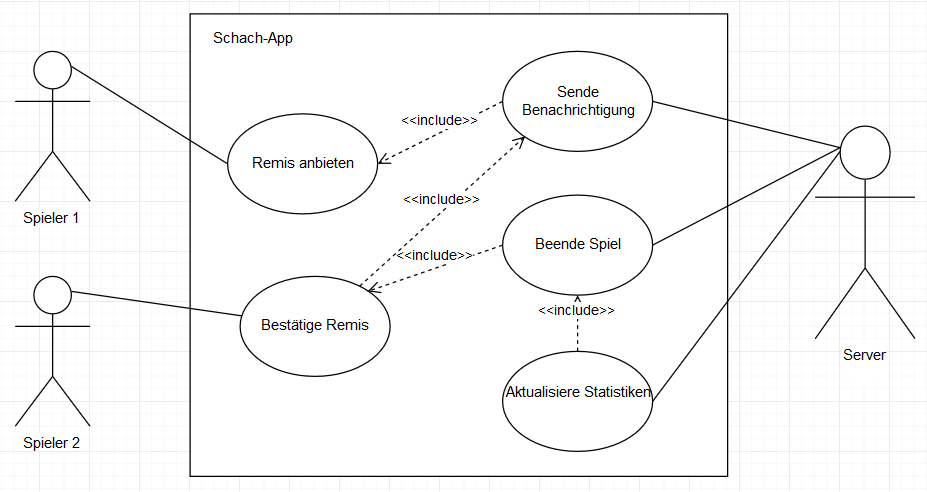
\includegraphics[width=1\linewidth]{Remis}
			\label{fig:remis}
			\captionof{figure}{Remis anbieten}
		\end{minipage}
\end{enumerate}

\glsaddall 
\printglossaries

\end{document}
